\documentclass[]{IEEEtran}
\IEEEoverridecommandlockouts
% The preceding line is only needed to identify funding in the first footnote. If that is unneeded, please comment it out.
\usepackage{amsmath,amssymb,amsfonts}
\usepackage{algorithmic}
\usepackage{graphicx,xcolor}
	\newcommand{\tB}{\textcolor{blue}}
	\newcommand{\tR}{\textcolor{red}}
	\newcommand{\tG}{\textcolor{green}}
	\newcommand{\bm}[1]{#1}
    % \newcommand{\tB}{\text}
	% \newcommand{\tR}{\text}
	% \newcommand{\tG}{\text}
\usepackage{textcomp}
\usepackage{cuted}
\usepackage{pgfplots}

\def\BibTeX{{\rm B\kern-.05em{\sc i\kern-.025em b}\kern-.08em
    T\kern-.1667em\lower.7ex\hbox{E}\kern-.125emX}}

\usepackage{cite}
\bibliographystyle{IEEEtran}

\usepackage{tikz}
\newtheorem{thm}{\bf Theorem}
\newtheorem{remark}{\bf Remark}
\newtheorem{assump}{\bf Assumption}
\newtheorem{lemma}{\bf Lemma}

\usepackage{arydshln}
    
\begin{document}

\title{The Fencing of Noncooperative Target by Single Integrators with Continuous Control Inspired by Super-Twisting Algorithm\\
\thanks{This work was partially supported by the National Key R\&D Program of China (Project No. 2020YFC2200800, Task No.2020YFC2200801), the National Natural Science Foundation of China (Grant No. 61703099), the Shenzhen Science and Technology Program, China (No. GXWD20201231165807008, 20200830220334001), and the funding for postdocs who have moved to Shenzhen, China.}
}

\author{
\IEEEauthorblockN{Cheng Liu, Fan Zhang}
\IEEEauthorblockA{\textit{School of Aeronautics and Astronautics} \\
\textit{Sun Yat-sen University} \\
Shenzhen, China \\
liuch586@mail2.sysu.edu.cn,\\
zhangfan6@mail.sysu.edu.cn}
\and
\IEEEauthorblockN{Xueyang Liao}
\IEEEauthorblockA{\textit{Department of GNC} \\
\textit{Institute of Guidance and Control} \\
Luoyang, China \\
664145669@qq.com
}
\and
\IEEEauthorblockN{Zezhou Zhang}
\IEEEauthorblockA{\textit{School of Mathematics and Big Data} \\
\textit{Anhui University of Science and Technology} \\
Huainan, China \\
3410438060@qq.com}
}

\maketitle

%TODO: 陈老师在非合作的目标下也是可以用的,文中做了一点对比。
\begin{abstract}
Bring Super-Twisting Algorithm to fencing problem
\end{abstract}

\begin{IEEEkeywords}
multiagent system, cooperative fencing, noncooperative target, singleton formation, nonsmooth analysis
\end{IEEEkeywords}

\section{Introduction}


This paper aims to preserve the advantages of the existing fencing control schemas
    and ensure a continuous control input.
Besides the highlighted label-free, flexible, fault-tolerant and local-frame-only features,
the contributions of our algorithm are:
\begin{enumerate}
    \item \textbf{Continuous Input}: The control input to the target is continuous.
\end{enumerate}

\newcommand{\NN}[0]{\mathbb{N}}
\newcommand{\RR}[0]{\mathbb{R}}
\def\closestpoint{P_{p_0}(p)}
% \newcommand{\ve}[2]{p_{{#1#2}}}
\newcommand{\ve}[2]{p_{{#1#2}}}
\newcommand{\norm}[1]{\left\lVert #1 \right\rVert}
\newcommand{\venorm}[2]{{\lVert p_{{#1#2}}\rVert}}
\newcommand{\dist}[2]{{\lVert p_{{#1#2}}\rVert}}
\newcommand{\veunit}[2]{\frac{p_{{#1#2}}}{\norm{p_{{#1#2}}}}}
\newcommand{\sgn}{\operatorname{sgn}}
\newcommand{\sig}[1]{\left\lfloor#1\right\rceil}
\newcommand{\Sgn}{\operatorname{Sgn}}
\newcommand{\sat}{\operatorname{sat}}
\newcommand{\dd}{\operatorname{d}}

\textit{Notations}:
Let $\NN \triangleq \{ 1, 2, \cdots, N \}$ represent the set of agents with the number $N \geq \tR{4}$.
The 2-norm of $p = [x,y]^T \in \RR^2$ is computed to be \( \norm{p} = \sqrt{ x^2 + y^2 } \). 
The unit vector associated with $p$ is defined as \( \sgn(p) = \frac{p}{\norm{p}} \) if \( \norm{p} \neq 0 \) and \( \sgn(p) = [0, 0]^T \) if \( \norm{p} = 0\).
The saturation operator is defined as $\sat_{\alpha}(p)=p$ if $\norm{p}\leq \alpha$ and $\sat_\alpha(p)=\alpha\sgn(p)$ if $\norm{p}>\alpha$.
Let $p_a \in \RR^2$ and $p_b \in \RR^2$, we denote $p_{ab} \triangleq p_a - p_b$.


\section{Problem Formation}

Consider the scenario where $N$ single integrators fence one target.
The agents' dynamics are
\begin{equation}\label{eq:agent}
    \dot{p}_i=u_{i}, \quad i\in \NN ,
\end{equation}
where \(p_i=[x_i,y_i]^T\) is the Cartesian coordinates of the $i$th agent.
$u_i$ is its velocity control input to be designed.
The noncooperative target's dynamic is
\begin{equation}\label{eq:target}   
    \dot{p}_0=u_0,
\end{equation}
where $p_0=[x_0,y_0]^T$ represents the target's position.

In this paper, we assume the input of the noncooperative target is 
bounded with 2-norm.
\tR{
\begin{assump}\label{assump:u0}
    The velocity control input of the target is Lipschitz continuous
    with Lipschitz constant $L$. 
\end{assump}
}
This means The derivative of the target's velocity is bounded with a given constant value $L$,
that is, $\Vert \dot{v}_0(t) \Vert \leq L, \forall\ t \geq 0$.

For analysis of the fencing agents' behavior, we denote the cluster's time-varying position by \( p= \left[ p_1^T, p_2^T, \cdots, p_N^T \right]^T \in \RR^{2N} \) and the region surrounded by agents with a convex hull defined as 
\begin{equation*}
    co(p) = \left\{ \sum_{i=1}^{N} \lambda_i p_i
    : \lambda_i \geq 0, \forall ~ i \in \NN 
    \text{ and } \sum_{i=1}^{N} \lambda_i = 1 \right\}.
\end{equation*}

As Fig. \ref{closest_distance} depicted, 
we define the distance between fencing agents and the target 
by 
\[
    dist(p_0, p) =
    \inf_{p^* \in co(p)} \norm{p_0 - p^*}.
\]
\begin{figure}[!ht]\label{closest_distance}
    \centering
    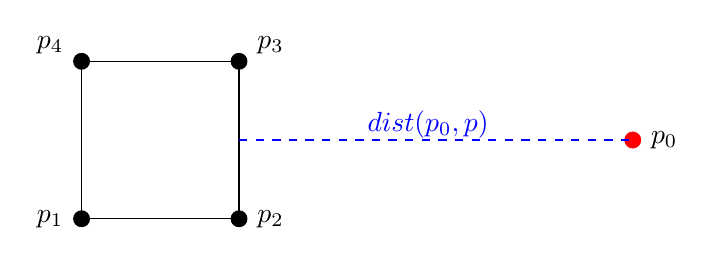
\begin{tikzpicture}
        % 跟随者当前位置
        \draw[] (3,0)--(5,0)--(5,2)--(3,2)--cycle;
        \filldraw (3,0) circle (.1)
        (5,0) circle (.1)
        (5,2) circle (.1)
        (3,2) circle (.1);
        \node at(2.6,0) {$p_1$};
        \node at(5.4,0) {$p_2$};
        \node at(5.4,2.2) {$p_3$};
        \node at(2.6,2.2) {$p_4$};
        % 跟随者目标位置
        % \draw[dotted] (8,0)--(10,0)--(10,2)--(8,2)--cycle;
        % \node at(7.6,0) {$p^*_1$};
        % \node at(10.4,0) {$p_2^*$};
        % \node at(10.4,2.2) {$p^*_3$};
        % \node at(7.6,2.2) {$p^*_4$};
        % 目标位置 
        \filldraw[red] (10,1) circle (.1);
        \node at(10.4,1) {$p_0$};
        % 目标轨迹
        \draw[blue, dashed] (5,1)--(10,1) node at(7.4,1.2) {$dist(p_0,p)$};
        % \filldraw[red] (10,1) circle (.07) node at(5.6,1.2) {\(\closestpoint\)};
    \end{tikzpicture}
    \caption{The fencing control problem with $4$ agents}
\end{figure}

Denote \( area(p) \) as the area of the convex hull \( co(p) \),
then the singleton formation (line formation) is the set  
\begin{equation}\label{singletonformation}
    \mathcal{S}_1 = \left\{ p \in\RR ^{2N} 
    | area(p) = 0 \right\}.
\end{equation}

Finally, the target-fencing problem can be defined as that
 $N$ agents \eqref{eq:agent} fence the target \eqref{eq:target}, 
 such that the closed-loop multiagent system satisfies the following properties:

\begin{enumerate}
    \item[P1] The agents asymptotically fence the target \( p_0 \) in the sense that \( \lim_{t \to \infty} dist(p_0, p) = 0 \);
    \item[P2] All agents keeps safety distance with respect to neighbors in the sense that $\| p_i(t) - p_j(t) \| > d$, $\forall ~ t \ge 0$, $i \neq j \in \NN$ for a designated $d > 0$;
    \item[P3] The final positions of all fencing agents do not lie in a singleton formation set \( \mathcal{S}_1 \), namely all agents are not stuck in a straight line.
    % \item[P4] No agent will be collapsed with the target in the sense that \(p_i\neq p_0,\forall i\in\NN,\forall t\geq 0\). 
\end{enumerate}

The communication network is defined as follows:
\begin{enumerate}
    \item Each agent can communicate with the agents within the range of communication distance $\mu$, and the relative displacement is measurable;
    \item At least one agent can measure the relative displacement to the target.
\end{enumerate}
Here, The neighbors are defined as 
\begin{equation}	\label{eq:Ni}
    \NN_i = \left\{ j \in \NN \ \big|\  \| p_j - p_i \| \le \mu \right\}.
\end{equation}
Define the communication graph as $\mathcal{G}(t)=\{\mathcal{V},\mathcal{E}\}$.
The nodes are all the label of agents $\mathcal{V}=\NN$ 
and the edges are dependent on the distance $\mathcal{E}=\{(i,j)\Vert i\in\NN,j\in\NN,\norm{p_{ij}}\leq \mu\}$.

Before moving on to the control strategies, one assumption is given as follows.

\begin{assump}	\label{assump:collision}
    Collision does not occur between any two agents at the initial time,
    that is $\| p_i(0) - p_j(0) \| > d$, $\forall ~ i \neq  j \in \NN$.
\end{assump}



\section{Main Results}

In this section, we present our results in two subsections.
The first subsection assumes the target's position is known to all agents.
The second subsection uses a distributed position observer to estimate the target's position under some assumptions.

\subsection{Fencing with Average Velocity Tracking}

The noncooperative target fencing control algorithm is formulated as
\begin{equation}\label{eq:sta}
    \begin{aligned}
        u_i &=- k_1 \sig{p_{i0}}^{1/2} + \phi_i   + v_i\\
        v_i &=- k_2 \sgn(p_{i0} )
    \end{aligned}, i \in \NN,
\end{equation}
where $k_1$ and $k_2$ is a positive constant gain value
which can be selected as $k_1>2 k_2+2 L + k_2 \gamma_2$, 
$\gamma_2>\frac{3 k_2 + 3L}{k_2-L}$ 
and $k_2>L$.
$- p_{i0}$ is the attractive term to track the target.
$\phi_i$ is the repulsive term from neighbors to keep safety distances.

The repulsive term $\phi_i$ is calculated with
\begin{equation}\label{eq:phiR}
    \phi_i = \sum_{ j \in \NN_i} \alpha_1 ( \dist{j}{i} ) \sgn( \ve{j}{i} ),
\end{equation}
where the set \( \NN_i \) is the set of agent $i$'s neighbors defined by \eqref{eq:Ni}
and the map \( \alpha : ( d, \infty ) \mapsto [ 0, \infty ) \) is a function satisfying
\begin{enumerate}
    \item[A1]  $\alpha_1(s) = 0$, $\forall ~ s \geq \mu$,
    \item[A2] \( \lim_{s \to d^+} \alpha_1(s) = \infty \), \label{A2}
\end{enumerate}

\begin{thm}
    The noncooperative-target fencing problem of single integrators \eqref{eq:agent} and
    the target \eqref{eq:target} with Super-Twisting Inspired algorithm \eqref{eq:sta} in the sense of P1-2
    under the Assumption \ref{assump:u0} and \ref{assump:collision}.
\end{thm}

\begin{IEEEproof}
    First, we write the error dynamics of the system as
    \begin{equation}\label{eq:error dynamic}
        \begin{aligned}
            \dot{r}_{i0} &=- k_1 \sig{p_{i0}}^{1/2} + \phi_i   + v_{i0}\\
            \dot{v}_{i0} &=- k_2 \sgn(p_{i0} ) - \dot{v}_0
        \end{aligned}, i \in \NN,
    \end{equation}
    Denote $e_i=p_{i0}$ and $z_i=v_{i0}/k1$, we obtain 
    \begin{equation}
        \begin{aligned}
            \dot{e}_i &= k_1 \left(-\sig{e_i}^{1/2}+z_i\right) + \phi_i \\
            \dot{z}_i &=\frac{k_2}{k_1} \left(-\sgn(e_i) - \frac{\dot{v}_0}{k_2}\right)
        \end{aligned}, i \in \NN,
    \end{equation}

    Inspired by \cite{chenDistributedFinitetimeDifferentiator2024},
    A Lyapunov function candidate is defined as:
    \begin{equation}
        V=V_0+ \gamma_1 V_1+ \gamma_2 V_2,
    \end{equation}
    where
    \begin{gather*}
        V_0=\sum_{i\in\NN} \left(-e_i^T z_i+\frac13 \norm{z_i}^3 + \frac23 k_1 \norm{e_i}^\frac32\right),\\
        V_1=\sum_{i\in\NN} \sum_{j\in\NN_i} 
        \int_{\norm{p_{ij}}}^\mu \alpha(s)\mathrm{d} s,\quad 
        V_2=\frac13 \sum_{i\in\NN} \norm{z_i}^3.
    \end{gather*}
    Obviously, $V_2$ is positive definite.
    Consider $V_0$, we have
    \begin{equation*}
        V_0\geq
        \sum_{i\in\NN} \left(
            -\norm{e_i} \norm{z_i}
            +\frac13 \norm{z_i}^3 + \frac23 \norm{e_i}^\frac32
            \right)\geq 0.
    \end{equation*}
    From the Young's inequality, we obtain
    % https://zhuanlan.zhihu.com/p/639167425
    \begin{equation*}
        \frac13 \norm{z_i}^3 + \frac23 \norm{e_i}^\frac32\geq \norm{e_i}\norm{z_i}
    \end{equation*}
    Then, $V$ is positive definite.
    
    Take the derivative of $V$ along the trajectory of the closed loop system, we find
    \begin{equation*}
        \dot{V}=\dot{V}_0+ \gamma_1 \dot{V}_1 + \gamma_2 \dot{V}_2,
    \end{equation*}
    where
    \begin{gather*}
        \dot{V}_0=\sum_{i\in\NN} \left(
            -z_i+ \sig{e_i}^\frac12
        \right)^T\dot{e}_i
        +\sum_{i\in\NN} \left(
            -e_i + \sig{z_i}^2
        \right)^T\dot{z}_i,\\
        \dot{V}_2=\sum_{i\in\NN} 
        \sig{z_i}^2 \cdot \dot{z}_i.
    \end{gather*}
    
    First, we consider the derivative of $V_0$.
    In the first term, we have
    \begin{equation*}
        \begin{aligned}
            &\left(
                -z_i+ \sig{e_i}^\frac12
            \right)^T\dot{e}_i\\
            =&\left(
                -z_i+ \sig{e_i}^\frac12
            \right)^T\left(
                -\sig{e_i}^\frac12+z_i+\phi_i
            \right)\\
            =&-\norm{z_i-\sig{e_i}^\frac12}^2
            -\left(z_i-\sig{e_i}^\frac12\right)^T\phi_i.
        \end{aligned}
    \end{equation*}
    In the second term, we find $\norm{\dot{z}_i}\leq \frac{k_2+L}{k_1}$.
    Then we obtain
    \begin{equation*}
        \begin{aligned}
        &\left(e_i-\sig{z_i}^2\right)^T\dot{z}_i \\
        \leq& \norm{e_i-\sig{z_i}^2} \norm{\dot{z}_i }
        \leq \frac{k_2}{k_1} \norm{e_i-\sig{z_i}^2} \\
        \leq& \frac{k_2+L}{k_1}
            \left(
            \norm{z_i}^2 + \norm{z_i -\sig{e_i}^\frac12 -z_i}^2
            \right)\\
        \leq& \frac{3 k_2+3 L}{k_1} \norm{z_i}^2 
        + \frac{2 k_2+2 L}{k_1} \norm{z_i-\sig{e_i}^\frac12}^2
        .
        \end{aligned}
    \end{equation*}
    As a result, we obtain 
    \begin{equation}\label{eq:V dot 12}
    \begin{aligned}
        \dot{V}_0
        \leq&
        -\left(1-\frac{2 k_2+2 L}{k_1}\right)  \norm{z_i-\sig{e_i}^\frac12}^2\\
        &+\frac{3 k_2+3 L}{k_1} \norm{z_i}^2 
        -\left(z_i-\sig{e_i}^\frac12\right)^T\phi_i
    \end{aligned}
    \end{equation}

    Similar to \cite{chenCooperativeTargetfencingProtocol2019}, we can take the derivative of $V_1$ as 
    \begin{equation*}
    \begin{aligned}
        \dot{V}_1&=-\sum_{i\in\NN} \phi_i^T \dot{e}_i\\
        &=-\sum_{i\in\NN} \left(z_i-\sig{e_i}^\frac12\right)^T\phi_i
        -\sum_{i\in\NN}\norm{\phi_i}^2  .
    \end{aligned}
    \end{equation*}

    Next, we consider the derivative of $V_2$
    \begin{equation*}\begin{aligned}
        \dot{V}_2
        =&\sum_{i\in\NN} \sig{z_i}^2 \cdot \dot{z_i}\\
        =& \frac{k_2}{k_1} \sum_{i\in\NN} \sig{z_i}^2 \cdot \left(-\sig{e_i}^0+\frac{\dot{v}_0}{k_2}\right)\\
        =& \frac{k_2}{k_1} \sum_{i\in\NN} \sig{z_i}^2 \cdot 
        \left(
            -\sig{z_i}^0+\frac{\dot{v}_0}{k_2}
            +\sig{z_i}^0-\sig{e_i}^0
        \right)\\
        =& -\frac{k_2}{k_1}(1-\frac{L}{k_2}) \sum_{i\in\NN} \norm{z_i}^2 
        + \frac{k_2}{k_1} \sum_{i\in\NN}\sig{z_i}^2 \cdot \left(
            \sig{z_i}^0-\sig{e_i}^0
            \right)
        .
    \end{aligned}
    \end{equation*}
    Let 
    $f_i=
    \norm{z_i-\sig{e_i}^\frac12}^2
    -\sig{z_i}^2 \cdot \left(
        \sig{z_i}^0-\sig{e_i}^0
    \right)$ with 
    $
    c=(\sig{z_i}^0\cdot\sig{e_i}^0) \in [-1,1]
    $
    Then, expand $f_i$ as
    \[\begin{aligned}
        f_i=&
        \norm{z_i}^2
        +\norm{e_i}
        -2\norm{z_i}\norm{e_i}^\frac12(\sig{z_i}^0\cdot\sig{e_i}^0)\\
        &-\norm{z_i}^2
        +\norm{z_i}^2 (\sig{z_i}^0\cdot\sig{e_i}^0)
        \\
        =&c\norm{z_i}^2
        +\norm{e_i}
        -2c\norm{z_i}\norm{e_i}^\frac12\\
        =&
        c \left(
            \norm{e_i}^\frac12-\norm{z_i}
        \right)^2 \geq 0
        .
    \end{aligned}
    \]
    So
    \[
        \sig{z_i}^2 \cdot \left(
            \sig{z_i}^0
            -\sig{e_i}^0
            \right)
        \leq 
        \norm{z_i-\sig{e_i}^\frac12}^2,
    \]
    and
    \begin{equation}
        \label{eq:V dot 3}
        \dot{V}_2 
        \leq -\frac{k_2-L}{k_1} \sum_{i\in\NN} \norm{z_i}^2
        + \frac{k_2}{k_1}  \sum_{i\in\NN} \norm{z_i -\sig{e_i}^\frac12}^2
        .
    \end{equation}
    Then
    \begin{equation*}
    \begin{aligned}
        \dot{V}
        \leq&
        -\left(1-\frac{2 k_2+2 L + k_2 \gamma_2}{k_1}\right)  
        \sum_{i\in\NN} \norm{z_i-\sig{e_i}^\frac12}^2\\
        &-(1+\gamma_1)\sum_{i\in\NN}  \left(z_i-\sig{e_i}^\frac12\right)^T\phi_i
        -\gamma_1\sum_{i\in\NN} \norm{\phi_i}^2\\
        &-\left(\frac{\gamma_2(k_2-L)}{k_1}-\frac{3 k_2+3 L}{k_1}\right) \sum_{i\in\NN} \norm{z_i}^2 \\
        =&
        -\sum_{i\in\NN}\norm{\frac{1+\gamma_1}{2\sqrt{\gamma_1}}(z_i-\sig{e_i}^\frac12)+\sqrt{\gamma_1}\phi_i}^2\\
        &-\left(\frac{\gamma_2(k_2-L)}{k_1}-\frac{3 k_2+3 L}{k_1}\right) \sum_{i\in\NN} \norm{z_i}^2 \\
    \end{aligned}
    \end{equation*}
    where 
    \begin{equation*}
        \gamma_1=\sqrt{\rho^2-1}+\rho,\quad
        \rho= 1-\frac{2 k_2+2 L + k_2 \gamma_2}{k_1}
    \end{equation*}
    Then, the system converges to the invariance set satisfying
    \begin{gather*}
            \frac{1+\gamma_1}{2\sqrt{\gamma_1}}(z_i-\sig{e_i}^\frac12)+\sqrt{\gamma_1}\phi_i=0,\\
            z_i=0.
    \end{gather*}
    As a result,
    \begin{equation}\label{eq:invariance}
        \sum_{i\in\NN}\sig{e_i}^\frac12
        =\sum_{i\in\NN}\frac{p_i-p_0}{\norm{e_i}^\frac12}
        =0.
    \end{equation}
    This implies 
    \begin{equation*}
        p_0=\sum_{i\in\NN}\lambda_i p_i \in Co(p).
    \end{equation*}
    Here, the $\lambda_i$ dependent on the position of agents.
    When no agent collapses with the target, we have 
    \begin{equation*}
        \lambda_i=
            \frac{\norm{e_i}^{-\frac12}}{\sum_{i\in\NN}\norm{e_i}^{-\frac12}}.
    \end{equation*}
    When there exists agents collapse with the target, we have
    \begin{equation*}
        \lambda_i=\begin{cases}
            \frac{\norm{e_i}^{-\frac12}}{\sum_{i\in\NN,e_i\neq 0}\norm{e_i}^{-\frac12}}, &e_i\neq 0;\\
            0,&e_i=0.
        \end{cases}
    \end{equation*}

\end{IEEEproof}

\subsection{Fencing with individual Velocity Tracking}

The noncooperative target fencing control algorithm is formulated as
\begin{equation}\label{eq:sta_individual}
    \begin{aligned}
        u_i &=- k_1 \sig{p_{i0}}^{1/2} + \phi_i   + v_i\\
        \dot{v}_i &=- k_2 \sgn(p_{i0} )+ \phi_i
    \end{aligned}, i \in \NN,
\end{equation}
where $k_1$ and $k_2$ is a positive constant gain value
which can be selected as $k_1>2 k_2+2 L + k_2 \gamma_2$, 
$\gamma_2>\frac{3 k_2 + 3L}{k_2-L}$ 
and $k_2>L$.
$- p_{i0}$ is the attractive term to track the target.
$\phi_i$ is the repulsive term from neighbors to keep safety distances.

\section{Simulation}

The results are very similar to \cite{kouCooperativeFencingControl2022} with enhancement on 
Through simulation, we found the tracking error cannot decay to zero.
The second controller can track the target's velocity as Fig. \ref{circle_individual_vi0}.
But the first controller cannot as Fig. \ref{circle_average_vi0}.

\tR{
    The simulation doesn't indicate the result as \eqref{eq:invariance}. So wierd!
}

\begin{figure}[htb]
    \includegraphics[width=\linewidth]{sta/circle_average.pdf}
    \caption{The fencing for noncooperative target with average velocity tracking}
\end{figure}

\begin{figure}[htb]
    \includegraphics[width=\linewidth]{sta/circle_individual.pdf}
    \caption{The fencing for noncooperative target with individual velocity tracking}
\end{figure}


\begin{figure}[htb]
    \includegraphics[width=\linewidth]{sta/circle_average_vi0.pdf}
    \caption{The fencing for noncooperative target with average velocity tracking}
    \label{circle_average_vi0}
\end{figure}

\begin{figure}[htb]
    \includegraphics[width=\linewidth]{sta/circle_individual_vi0.pdf}
    \caption{The fencing for noncooperative target with individual velocity tracking}
    \label{circle_individual_vi0}
\end{figure}


\bibliography{/home/xsr/repo/texes/bin/我的文库.bib}

\end{document}